\documentclass[10pt,conference]{IEEEtran}
\usepackage{cite}
\usepackage{float}
\usepackage{minted}
\usepackage[T1]{fontenc}
\usepackage[utf8]{inputenc}
\ifCLASSINFOpdf
   \usepackage[pdftex]{graphicx}
   \graphicspath{{figs/}}
   \DeclareGraphicsExtensions{.pdf,.jpeg,.png}
\else
   \usepackage[dvips]{graphicx}
   \graphicspath{{../figs/}}
   \DeclareGraphicsExtensions{.eps}
\fi
\usepackage[cmex10]{amsmath}
\interdisplaylinepenalty=2500
\usepackage{amsthm}
\newtheorem{definition}{Definition}
\usepackage{algorithmic}
\usepackage{array}
\ifCLASSOPTIONcompsoc
  \usepackage[caption=false,font=normalsize,labelfont=sf,textfont=sf]{subfig}
\else
  \usepackage[caption=false,font=footnotesize]{subfig}
\fi
\usepackage{url}
\hyphenation{op-tical net-works semi-conduc-tor}
\usepackage[left=1.6cm,top=4cm,right=1.6cm,bottom=1.5cm,headheight=1cm]{geometry}
\usepackage{lipsum}
\usepackage{graphicx}
% utilizado para calcular o tamanho da pagina
\usepackage{tikz}
\usepackage{fancyhdr}
\usepackage{tikzpagenodes}
\renewcommand{\headrulewidth}{0pt}
\renewcommand{\footrulewidth}{0pt}
\usetikzlibrary{calc}
\pagestyle{fancy}
\setlength\headheight{12.0pt}
\addtolength{\textheight}{-42.0pt}
\addtolength{\topmargin}{-2.0pt}

\fancyhead[L]{\begin{tikzpicture}[remember picture,overlay]
\draw  let \p1=($(current page.north)-(current page header area.south)$),
      \n1={veclen(\x1,\y1)} in
node [inner sep=0,outer sep=0,below right] 
      at (current page.north west){
\includegraphics[width=\paperwidth,height=\n1]{headerimg.png}};
\end{tikzpicture}}

\fancyfoot[R]{\begin{tikzpicture}[remember picture,overlay]
\draw  let \p1=($(current page footer area.north)-(current page.south)$),
      \n1={veclen(\x1,\y1)} in
node [inner sep=0,outer sep=0,above right] 
      at (current page.south west){
\includegraphics[width=\paperwidth,height=\n1]{footerimg.png}};
\end{tikzpicture}}

\begin{document}
\title{Weed and Anomaly Detection in Maize Fields with Deep Learning on Fragmented Orthomosaics}
\newif\iffinal
\finaltrue
\iffinal
    % \author{
    % \IEEEauthorblockN{Vinicius Tessele}
    % \IEEEauthorblockA{Dept. of Artificial Intelligence \\
    % Biopark Educação \\
    % Toledo, Brazil \\
    % ORCID: 0000-0002-0662-9200}
    % \and
    % \IEEEauthorblockN{Claudio Honorio da Silva Junior}
    % \IEEEauthorblockA{Dept. of Artificial Intelligence \\
    % Biopark Educação \\
    % Toledo, Brazil \\
    % ORCID: 0009-0000-5043-0517}
    % \and
    % \IEEEauthorblockN{Angelo Gabriel}
    % \IEEEauthorblockA{Dept. of Artificial Intelligence \\
    % Biopark Educação \\
    % Toledo, Brazil \\
    % ORCID: 0009-0005-7939-5301}
    % \and
    % \IEEEauthorblockN{Leonardo Tampelini}
    % \IEEEauthorblockA{Dept. of Artificial Intelligence \\
    % Biopark Educação \\
    % Toledo, Brazil \\
    % ORCID: 0009-0000-9307-4444}
    % }
\else
  \author{ID do artigo Latin.science 2020: \cmtid \\ }
\fi
\maketitle
\thispagestyle{fancy}

\begin{abstract}
This work presents the development of a computer vision pipeline for detecting anomalies in maize crops, including weeds, planting gaps, and overlapping plants. The initial dataset consisted of high-resolution orthomosaic images provided by a partner company. Due to their large size and complexity, these images were segmented into 600×600 pixel tiles, resulting in 1,316 sub-images. After assessing quality, 451 images were selected and manually annotated using a custom labeling tool developed with Pygame. Initially, the Weeds-Galore dataset and DeepLabv3 model were explored, but due to limited performance, the approach was shifted to YOLO-based object detection. The annotated dataset was divided into training, validation, and test sets, with a recommended 70/15/15 distribution. The proposed solution aims to support agricultural monitoring by automating anomaly detection in large-scale crop imagery.
\end{abstract}

\renewcommand{\IEEEkeywordsname}{Keywords}
\begin{IEEEkeywords}
computer vision, weed detection, orthomosaic, maize crop, deep learning, YOLO, image labeling, agricultural monitoring
\end{IEEEkeywords}

\renewcommand{\abstractname}{Resumo}

\begin{abstract}
Este trabalho apresenta o desenvolvimento de um pipeline de visão computacional para a detecção de anomalias em lavouras de milho, incluindo plantas daninhas, falhas no plantio (gaps) e plantas sobrepostas. O conjunto inicial de dados consistia em imagens ortomosaicas de alta resolução fornecidas por uma empresa parceira. Devido ao tamanho e complexidade das imagens, estas foram divididas em subimagens de 600×600 pixels, resultando em 1.316 imagens. Após avaliação de qualidade, 451 imagens foram selecionadas e anotadas manualmente com uma ferramenta de rotulagem desenvolvida em Pygame. Inicialmente, foi explorado o uso do conjunto de dados Weeds-Galore e do modelo DeepLabv3, mas devido à performance limitada, a abordagem foi direcionada para a detecção de objetos baseada em YOLO. O conjunto anotado foi dividido em conjuntos de treino, validação e teste, com uma distribuição recomendada de 70\% treino, 15\% validação e 15\% teste. A solução proposta visa apoiar o monitoramento agrícola, automatizando a detecção de anomalias em imagens de grandes áreas de cultivo.
\end{abstract}

\renewcommand\IEEEkeywordsname{Palavras-chave}

\begin{IEEEkeywords}
visão computacional, detecção de plantas daninhas, ortomosaico, lavoura de milho, deep learning, YOLO, rotulagem de imagens, monitoramento agrícola
\end{IEEEkeywords}

\IEEEpeerreviewmaketitle

\section{Introdução} 

A Inteligência Artificial (IA) tem transformado profundamente a forma como interagimos com a tecnologia e com o mundo ao nosso redor. Desde assistentes virtuais até sistemas de recomendação e carros autônomos, os avanços nessa área têm proporcionado ganhos significativos em eficiência, produtividade e inovação. No entanto, esse crescimento acelerado levanta questões importantes sobre ética, responsabilidade e impactos sociais da IA, que precisam ser considerados com igual atenção \cite{garcia2020ia, pinto2020responsabilidade}.

O uso de IA no setor agrícola é um exemplo claro de como essas tecnologias podem ser aplicadas em contextos práticos para solucionar problemas reais. Técnicas de aprendizado profundo, como as redes neurais convolucionais (CNNs), têm se mostrado eficazes na identificação de doenças em plantas, otimizando processos e reduzindo perdas na produção agrícola \cite{kamilaris2018deep, dosSantos2020segmentacao}. Essas soluções automatizadas tornam-se cada vez mais viáveis com o avanço dos modelos de detecção de objetos, como o YOLO (You Only Look Once), que permite reconhecimento em tempo real com alta precisão \cite{zhao2019object, redmon2018yolov3}.
\begin{figure}[!ht]
\centering
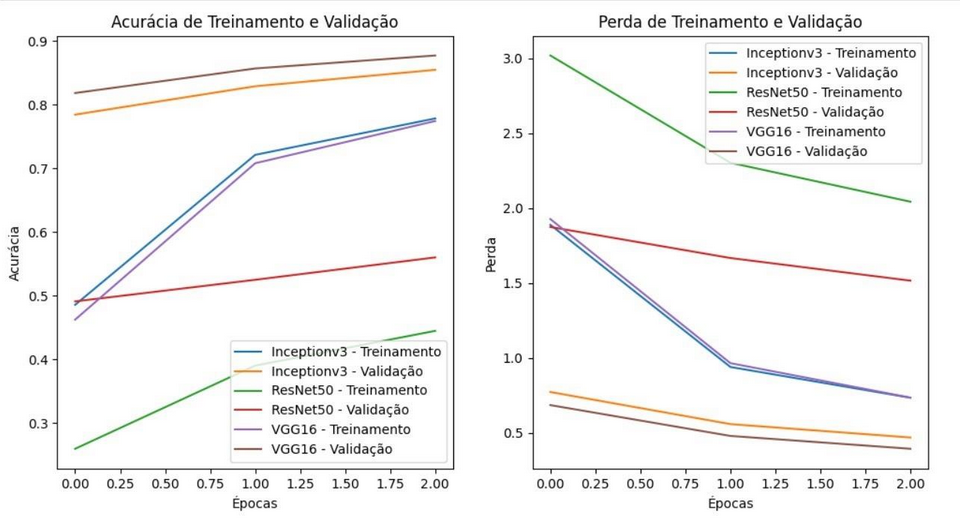
\includegraphics[width=0.8\linewidth]{fig001.png}
\caption{Foto panoramica da plantacao de milho}
\label{fig:fig01}
\end{figure}

A Figura~\ref{fig:fig01} apresenta uma imagem panorâmica da plantação de milho, ilustrando o tipo de cenário analisado neste trabalho.

No entanto, a aplicação da inteligência artificial na agricultura também levanta preocupações importantes, especialmente no que diz respeito à equidade social, sustentabilidade ética e inclusão tecnológica. A adoção de tecnologias avançadas, como a visão computacional e o aprendizado profundo, pode acentuar desigualdades já existentes entre grandes produtores – que possuem maior acesso a infraestrutura, conectividade e conhecimento técnico – e pequenos agricultores, que enfrentam barreiras econômicas e educacionais significativas. A lacuna digital no campo pode, assim, se tornar um entrave à democratização dos benefícios da IA.

Além disso, a ausência de regulamentações robustas sobre o uso de IA em contextos agrícolas levanta questões críticas sobre privacidade de dados georreferenciados, responsabilidade em decisões automatizadas (por exemplo, em sistemas de pulverização autônoma) e a transparência dos modelos de machine learning utilizados – frequentemente tratados como caixas-pretas. Como apontado por Mittelstadt et al. (2016), os sistemas automatizados exigem estruturas de governança ética que assegurem não apenas desempenho técnico, mas também justiça, explicabilidade e responsabilidade social \cite{mittelstadt2016ethics}. Nesse contexto, é fundamental que o desenvolvimento e a implementação dessas tecnologias considerem uma abordagem participativa e centrada no ser humano, buscando garantir que os avanços da IA na agricultura beneficiem toda a cadeia produtiva de forma justa e sustentável.
\begin{figure}[!ht]
\centering
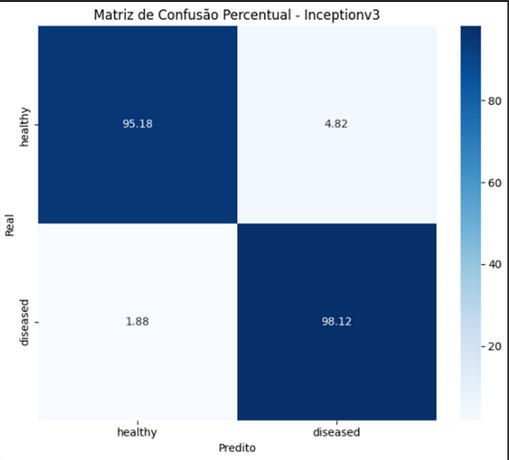
\includegraphics[width=0.8\linewidth]{fig002.png}
\caption{Gaps & Plantas duplas}
\label{fig:fig02}
\end{figure}

A Figura~\ref{fig:fig02} exemplifica a segmentação manual da plantação, destacando gaps e plantas sobrepostas, que são desafios importantes para o processamento automático das imagens.

\section{Trabalhos Relacionados}

\subsection{Detecção e Segmentação de Plantas Daninhas: WeedsGaloRe}

A detecção automatizada de plantas daninhas em culturas agrícolas tem sido amplamente estudada como uma aplicação importante da inteligência artificial na agricultura de precisão. O conjunto de dados \textit{WeedsGaloRe} tem se destacado como um benchmark relevante para o treinamento e avaliação de modelos de segmentação e detecção de plantas daninhas em imagens aéreas e de campo \cite{dosSantos2020segmentacao}. Essa base de dados foi desenvolvida a partir de imagens capturadas em lavouras de milho, contendo anotações precisas das áreas afetadas por plantas invasoras, o que permite o desenvolvimento de modelos robustos e específicos para o contexto agrícola.
\begin{figure}[!ht]
\centering
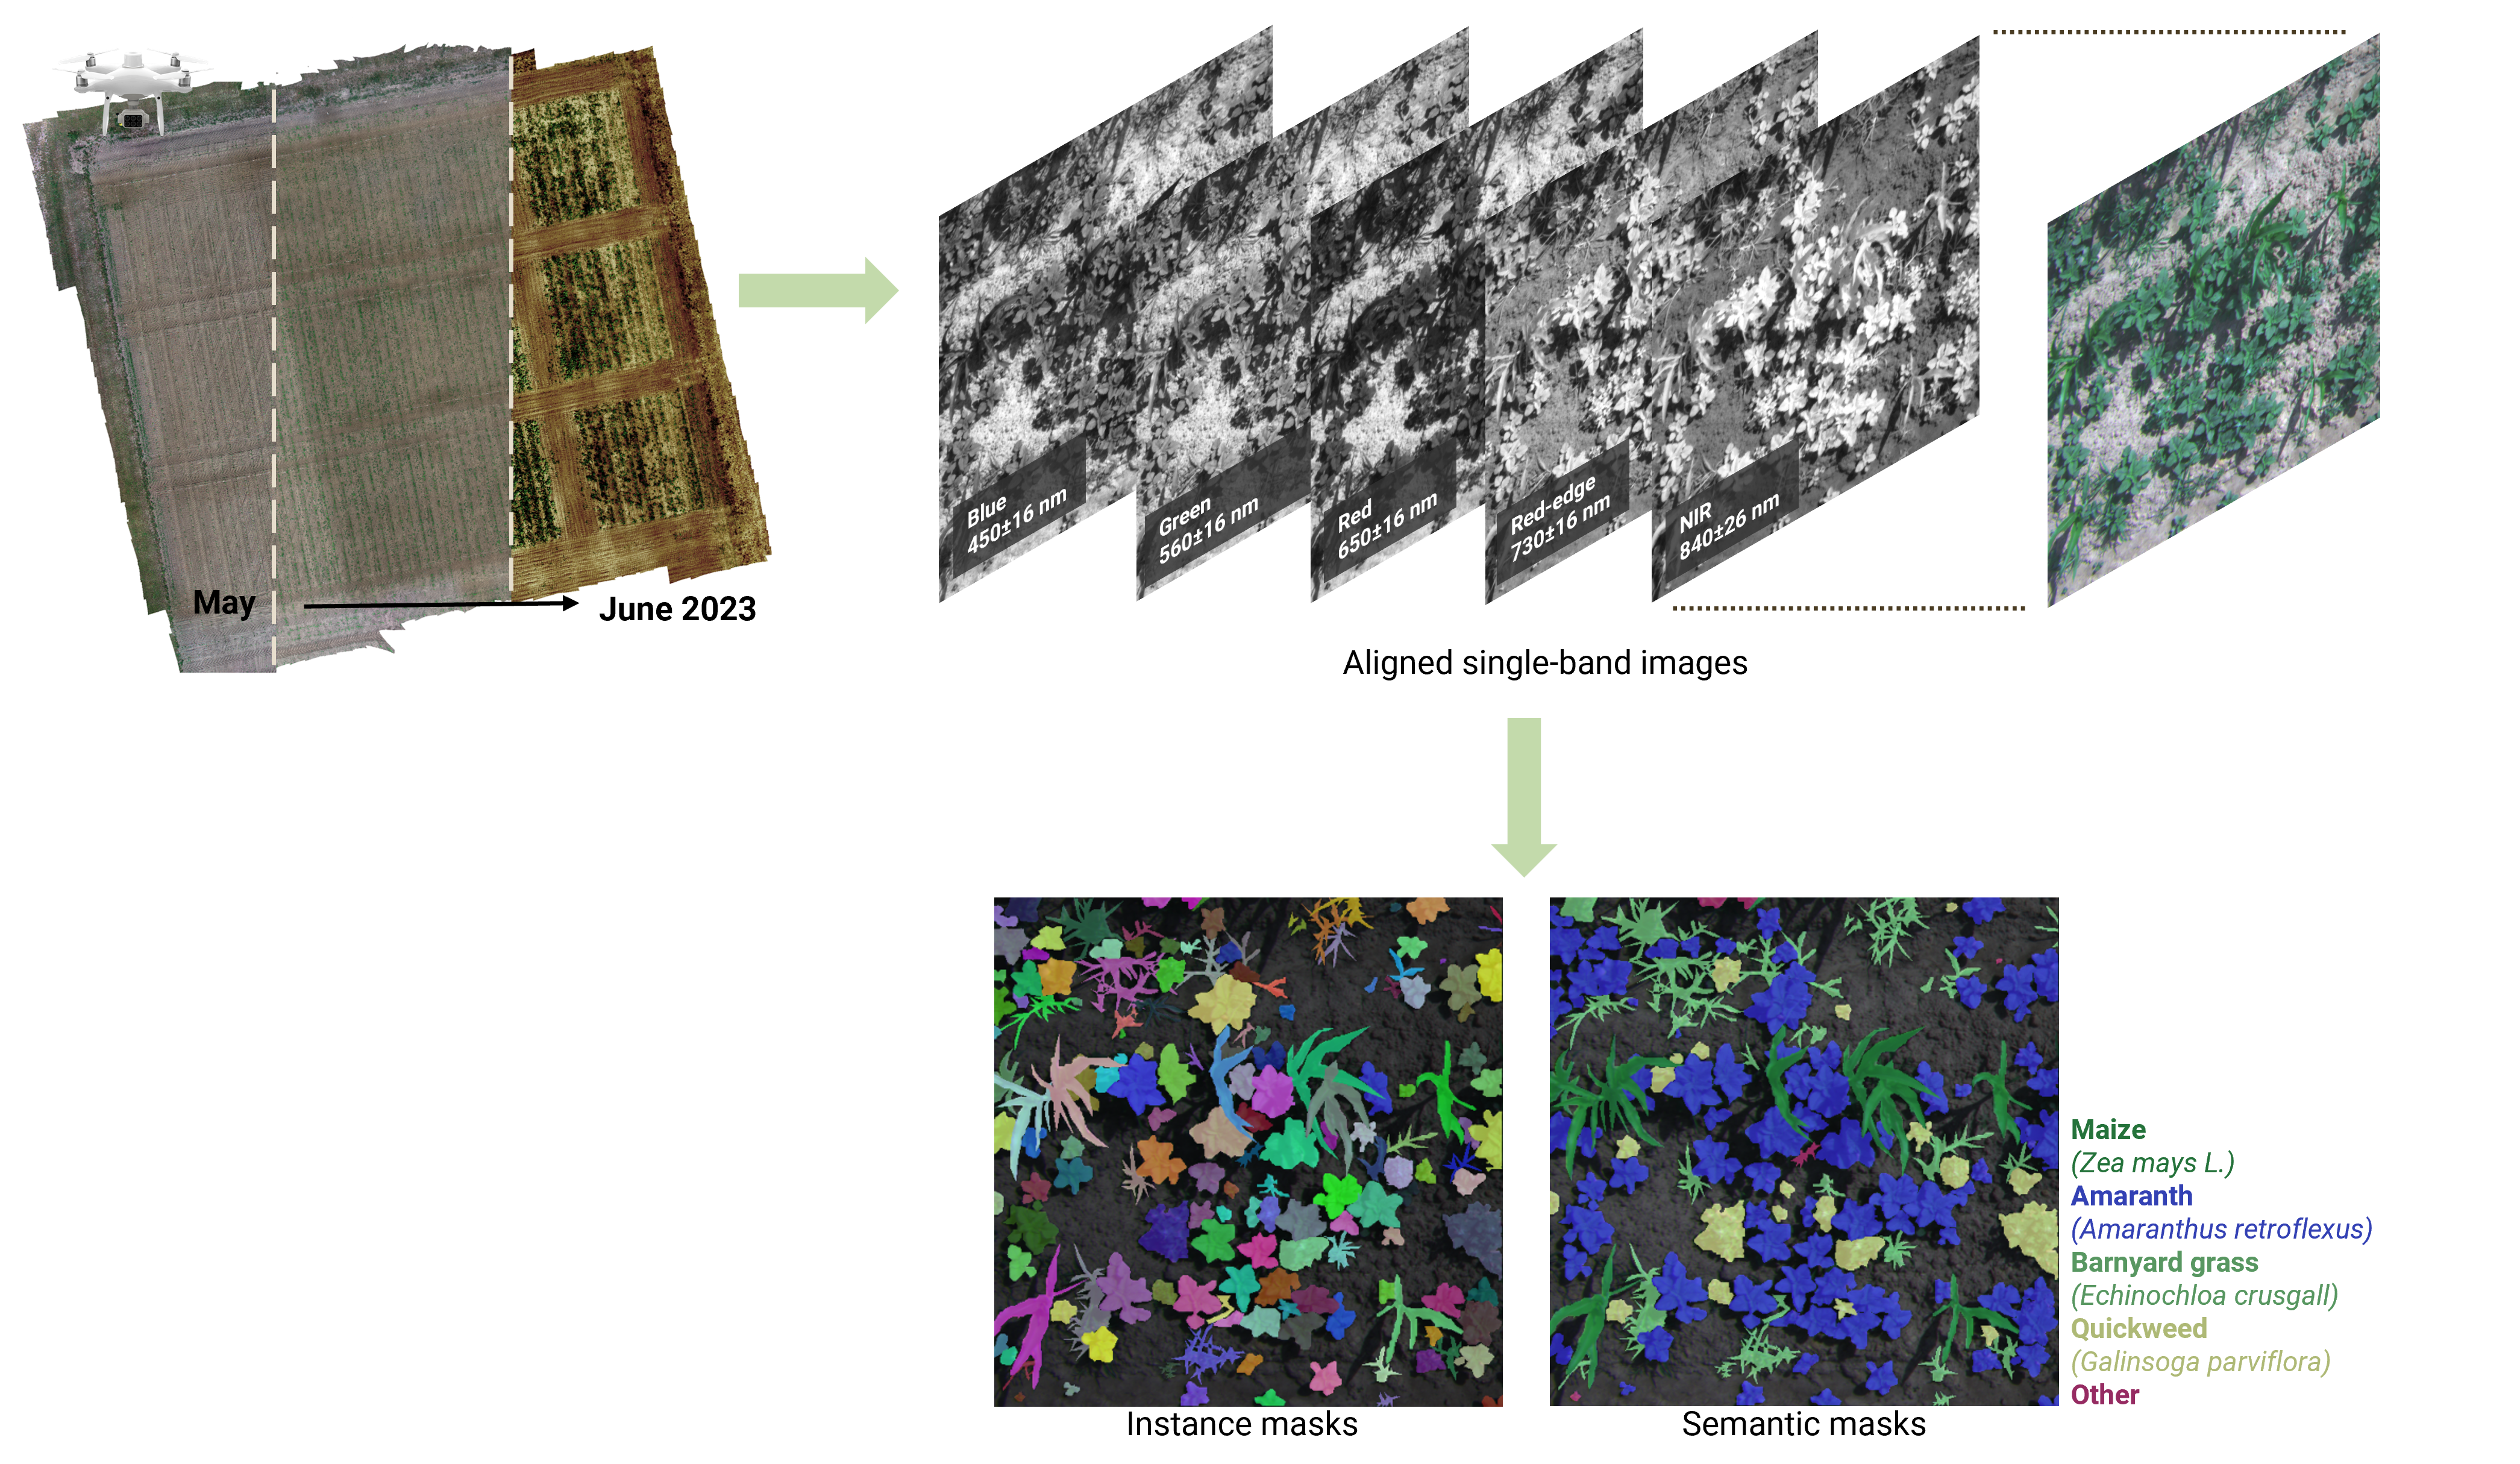
\includegraphics[width=0.8\linewidth]{fig003.png}
\caption{Exemplo de imagem da base WeedsGaloRe com segmentação de plantas daninhas.}
\label{fig:weedsgalore_sample}
\end{figure}

Apesar dos avanços, desafios como a variabilidade visual das plantas daninhas, condições ambientais e a qualidade das imagens dificultam o desempenho dos modelos, o que demanda o desenvolvimento contínuo de arquiteturas de redes neurais profundas e técnicas de pré-processamento de imagens.

\subsection{Redes Neurais Convolucionais (CNNs) na Contagem e Detecção de Plantas}

Redes neurais convolucionais (CNNs) têm sido a principal abordagem para tarefas de reconhecimento, segmentação e contagem de plantas em imagens agrícolas. Modelos populares como \textit{YOLOv5} e \textit{EfficientNet} têm demonstrado eficiência no processamento rápido e preciso de imagens de alta resolução, permitindo a identificação de múltiplos objetos (plantas, plantas daninhas, falhas) em tempo real \cite{zhao2019object, redmon2018yolov3, kamilaris2018deep}.

Em particular, trabalhos recentes têm focado no uso dessas arquiteturas para quantificar o número de plantas e identificar anomalias, como sobreposições e gaps, melhorando a precisão do monitoramento das lavouras e auxiliando na tomada de decisão agrícola \cite{dosSantos2020segmentacao}. Técnicas de \textit{data augmentation}, \textit{transfer learning} e uso de datasets anotados manualmente têm sido essenciais para superar a escassez de dados rotulados específicos para o milho.

\subsection{Uso de Orto-mosaicos e OpenStreetMap na Agricultura de Precisão}

A geração de ortomosaicos, que são imagens aéreas ortorretificadas e compostas a partir de múltiplos mosaicos, é uma prática consolidada para o monitoramento de áreas agrícolas extensas. A integração desses dados com sistemas de informações geográficas (SIG), especialmente utilizando ferramentas como o \textit{OpenStreetMap}, permite a geolocalização precisa dos elementos da lavoura, facilitando o mapeamento, análise e planejamento agronômico \cite{kamilaris2018deep}.

Esse tipo de abordagem tem sido fundamental para a agricultura de precisão, pois possibilita o desenvolvimento de aplicações que simulam o sobrevoo de drones para inspeção contínua, permitindo a identificação em tempo real de plantas daninhas, falhas no plantio e outras anomalias no campo.

\subsection{Rotulagem Manual e Uso de Pygame para Criação de Datasets}

A construção de datasets anotados é uma etapa crítica para o treinamento de modelos de \textit{deep learning}, sobretudo em domínios específicos como a agricultura, onde conjuntos de dados públicos são escassos ou insuficientes. Ferramentas simples e customizáveis, como o \textit{Pygame}, têm sido utilizadas para desenvolver aplicações de rotulagem manual de imagens~\ref{fig:fig04}, facilitando a criação de anotações precisas e adaptadas às necessidades do projeto \cite{tessele2024modelo}.
\begin{figure}[!ht]
\centering
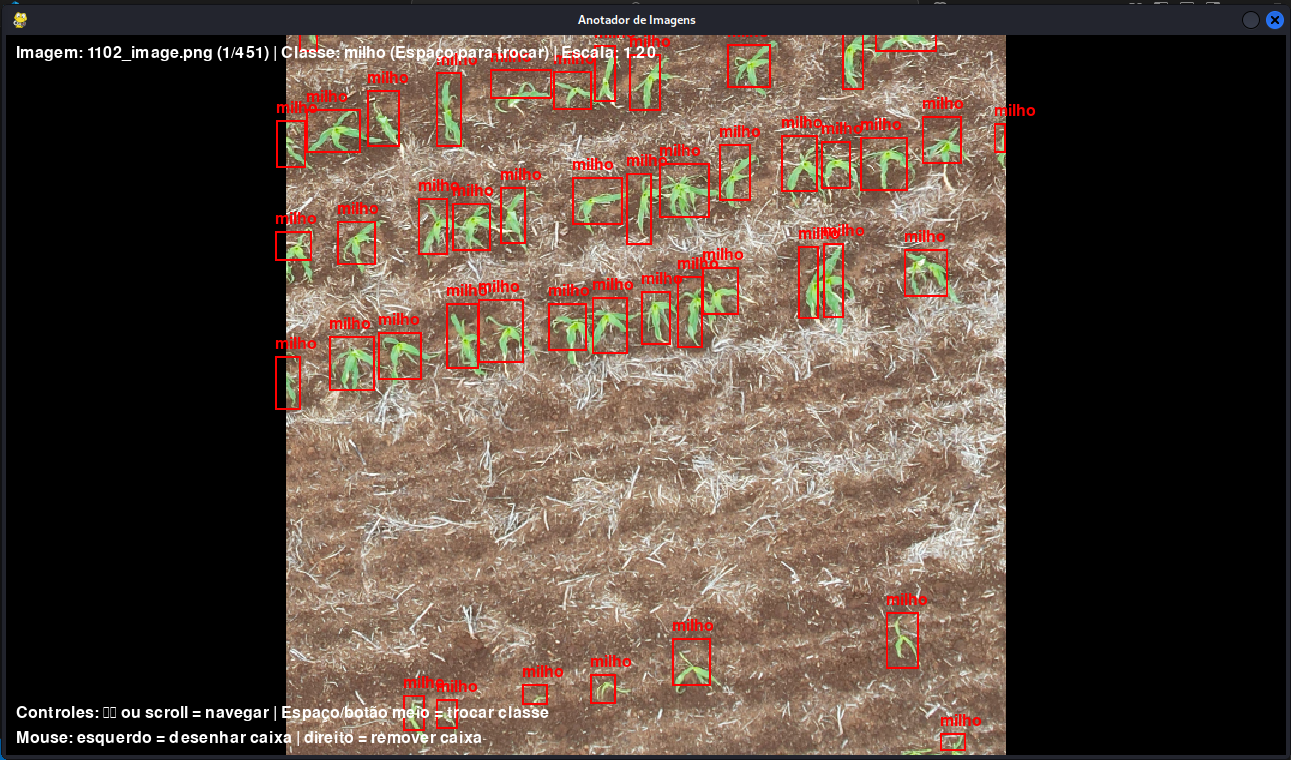
\includegraphics[width=0.8\linewidth]{fig004.png}
\caption{App Criado para rotulagens de imagens com pygame}
\label{fig:fig04}
\end{figure}
O uso de interfaces gráficas interativas para \textit{labeling} não só acelera o processo, mas também melhora a qualidade das anotações, impactando diretamente na performance dos modelos de detecção. Essa abordagem tem se mostrado eficiente para preparar bases de dados específicas para detecção de plantas daninhas, contagem de plantas e identificação de falhas em culturas como o milho.

\section{Resultados}
\subsection{Precisão da CNN para detecção de milho}
ok
\subsection{Precisão da CNN binária milho vs não-milho}
\subsection{Simulação da contagem e identificação em ortomosaico}
\subsection{Discussão sobre performance em diferentes resoluções ou tipos de terreno}

\section{Discussão e Trabalhos Futuros}
\subsection{Inserção da CNN em tempo real em drones reais}
\subsection{Aplicação de georreferenciamento para identificação de regiões críticas}
\subsection{Aumento do dataset com dados sintéticos}
\subsection{Discussão ética: automação, impacto social}

\bibliographystyle{IEEEtran}
\bibliography{bibliografia}

\end{document}